% !TEX root = saveliev_physics_general_course_1.tex
%!TEX TS-program = pdflatex
%!TEX encoding = UTF-8 Unicode


\chapter{CÁC HỆ QUY CHIẾU PHI QUÁN TÍNH}\label{chap:4}

\section{Các lực quán tính}\label{sec:4_1}

Các định luật Newton chỉ đúng trong các hệ quy chiếu quán tính. Đối với tất cả các hệ quy chiếu quán tính, vật đã cho chuyển động với cùng gia tốc $a$. Một hệ quy chiếu phi quán tính bất kỳ chuyển động đối với các hệ quy chiếu quán tính khác với gia tốc nào đó, do đó gia tốc $\vec{a}'$ của một vật trong hệ quy chiếu phi quán tính sẽ khác  $\vec{a}$. Gọi $\vec{a}_0$ là hiệu số các gia tốc của vật trong hệ quy chiếu quán tính và phi quán tính:
\begin{equation}\label{eq:4_1}
\vec{a} - \vec{a}' = \vec{a}_0.
\end{equation}

\noindent
Đối với hệ quy chiếu phi quán tính chuyển động tịnh tiến, $\vec{a}_0$ là như nhau đối với mọi điểm trong không gian ($\vec{a}_0=\text{const}$) và là gia tốc của hệ quy chiếu phi quán tính. Đối với hệ quy chiếu quán tính quay, $\vec{a}_0$ sẽ khác nhau đối với các điểm khác nhau trong không gian [$\vec{a}_0=\vec{a}_0(\vec{r}')$, với $\vec{r}'$ là vector vị trí xác định vị trí của một điểm đối với hệ quy chiếu phi quán tính].

Giả sử tổng hợp các lực do các vật khác tác dụng lên vật là $\vec{F}$. Khi đó, theo định luật II Newton, gia tốc của vật so với bất kỳ hệ quy chiếu quán tính nào là
\begin{equation*}
\vec{a} = \frac{1}{m}\vec{F}.
\end{equation*}

\noindent
Theo \eqn{4_1}, gia tốc của vật này đối với hệ quy chiếu phi quán tính được biểu diễn dưới dạng
\begin{equation*}
\vec{a}' = \vec{a} - \vec{a}_0 = \frac{1}{m}\vec{F} - \vec{a}_0.
\end{equation*}

\noindent
Từ đây suy ra rằng ngay cả khi $\vec{F}=0$, vật vẫn sẽ chuyển động với gia tốc $-\vec{a}_0$ đối với hê quy chiếu phi quán tính, hay nói cách khác, như là có một lực bằng $-m\vec{a}_0$ tác dụng lên vật.

Điều nói trên có nghĩa là ta có thể dùng các phương trình Newton để mô tả chuyển động trong các hệ quy chiếu phi quán tính, nếu ngoài các lực do các vật tác dụng với nhau, ta tính cả các lực được gọi là\textbf{các lực quán tính} $\vec{F}_{\text{in}}$. Ta giả thiết rằng các lực quán tính bằng với tích của khối lượng vật và hiệu các gia tốc so với hệ quy chiếu quán tính và phi quán tính lấy với dấu ngược lại:
\begin{equation}\label{eq:4_2}
\vec{F}_{\text{in}} = -m(\vec{a} - \vec{a}') = -m\vec{a}_0.
\end{equation}

\begin{figure}[!htb]
	\begin{center}
		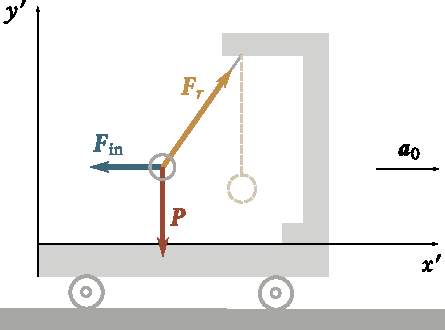
\includegraphics[scale=0.95]{figures/ch_04/fig_4_1.pdf}
		\caption[]{}
		\label{fig:4_1}
	\end{center}
\end{figure}

\noindent
Một cách tương ứng, phương trình định luật II Newton đối với hệ quy chiếu phi quán tính sẽ có dạng
\begin{equation}\label{eq:4_3}
m\vec{a}' = \vec{F} + \vec{F}_{\text{in}}.
\end{equation}

Ta hãy làm sáng tỏ khẳng định của chúng ta bằng ví dụ sau đây. Xét một chiếc xe nhỏ có một giá đỡ gắn chặt vào xe; một quả cầu nhỏ được treo vào giá bằng một sợi dây (\fig{4_1}). Khi xe đứng yên hoặc chuyển động không có gia tốc, sợi dây sẽ ở vị trí thẳng đứng, và trọng lực $\vec{P}$ cân bằng với phản lực của sợi dây $\vec{F}_{\text{r}}$. Bây giờ chúng ta cho chiếc xe chuyển động tịnh tiến với gia tốc $\vec{a}_0$. Sợi dây sẽ lệch khỏi phương thẳng đứng một góc sao cho tổng hợp của các lực $\vec{P}$ và $\vec{F}_{\text{r}}$ truyền cho quả cầu một gia tốc $\vec{a}_0$. Quả cầu sẽ ở trạng thái nghỉ so với hệ quy chiếu gắn với xe, mặc dù tổng hợp của các lực $\vec{P}$ và $\vec{F}_{\text{r}}$ khác không. Sự không có mặt của gia tốc quả cầu so với hệ quy chiếu này có thể được giải thích một cách hình thức là, ngoài các lực $\vec{P}$ và $\vec{F}_{\text{r}}$ có tổng bằng $m\vec{a}_0$, lực quán tính $\vec{F}_{\text{in}}=-m\vec{a}_0$ còn tác dụng lên quả cầu.

Việc đưa vào các lực quán tính cho phép chúng ta mô tả chuyển động của các vật trong hệ quy chiếu (quán tính cũng như phi quán tính) bất kỳ bằng các phương trình chuyển động giống nhau.

Cần hiểu rõ rằng các lực quán tính không thể được xem như cùng loại với các lực đàn hồi, lực hấp dẫn, và lực ma sát, hay nói cách khác, các lực do các vật khác tác dụng lên vật. Các lực quán tính được gây ra bởi các tính chất của hệ quy chiếu trong đó các hiện tượng cơ học được nghiên cứu. Với nghĩa này, chúng có thể được gọi là các lực ảo.

Việc đưa vào xét các lực quán tính là không cần thiết. Về nguyên tắc, bất kỳ chuyển động nào cũng có thể được xét đối với hệ quy chiếu quán tính. Tuy nhiên trên thực tế, chuyển động của các vật đối với các hệ quy chiếu phi quán tính, chẳng hạn đối với mặt đất, thường có ý nghĩa thực sự. Việc sử dụng các lực quán tính sẽ giúp giải trực tiếp bài toán tương ứng đối với một hệ quy chiếu, và điều đó thường đơn giản hơn rất nhiều so với việc nghiên cứu chuyển động trong một hệ quy chiếu quán tính.

\begin{figure}[!htb]
	\begin{center}
		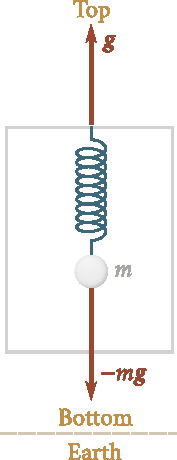
\includegraphics[scale=0.85]{figures/ch_04/fig_4_2.pdf}
		\caption[]{}
		\label{fig:4_2}
	\end{center}
\end{figure}

Một tính chất đặc trưng của các lực quán tính là chúng tỷ lệ thuận với khối lượng của vật. Nhờ tính chất này mà các lực quán tính giống như các lực hấp dẫn. Tưởng tượng chúng ta đang ở trong một cái buồng kín, xa tất cả các vật bên ngoài và đang chuyển động thẳng đứng với gia tốc $\vec{g}$ theo hướng mà ta gọi là hướng ``trên'' (\fig{4_2}). Khi đó các vật bên trong buồng đều chuyển động như thể có lực quán tính $-m\vec{g}$ tác dụng lên chúng. Nói riêng, một lò xo mà ở một đầu của nó được treo cố định một vật có khối lượng $m$ sẽ dãn ra sao cho lực đàn hồi cân bằng với lực quán tính $-m\vec{g}$. Tuy nhiên, ta có thể quan sát được hiện tượng tương tự khi buồng đứng yên và nằm gần bề mặt Trái Đất. Nếu không có khả năng ``nhìn'' ra bên ngoài buồng thì không thể thông qua bất kỳ thí nghiệm nào thực hiện trong buồng mà ta có thể phát hiện được lực $-m\vec{g}$ được gây ra bởi chuyển động có gia tốc của buồng hay do tác dụng của trường hấp dẫn của Trái Đất. Trên cơ sở này người ta nói về sự tương đương giữa các lực quán tính và trọng lực. Sự tương đương này là cơ sở của thuyết tương đối rộng của Albert Einstein.

\section{Lực quán tính ly tâm}\label{sec:4_2}

Ta hãy xét một cái đĩa quay xung quanh trục thẳng đứng $z'$ vuông góc với đĩa với vận tốc góc $\omega$ (\fig{4_3}). Một quả cầu được xuyên vào một cái nan hoa và nối với tâm đĩa bằng một lò xo, quay cùng với đĩa. Quả cầu chiếm trên nan hoa một vị trí mà ở đó lực đàn hồi $\vec{F}_{\text{spr}}$ của lò xo bằng tích của khối lượng $m$ của quả cầu với gia tốc $\vec{a}_n = -\omega^2R$ của nó [see \eqn{1_102}; $\vec{R}$ là vector vị trí vẽ từ tâm đĩa tới quả cầu, module $R$ của nó cho khoảng cách của quả cầu tính từ tâm đĩa]:
\begin{equation}\label{eq:4_4}
\vec{F}_{\text{spr}} = -m\omega^2\vec{R}.
\end{equation}

\begin{figure}[!htb]
	\begin{center}
		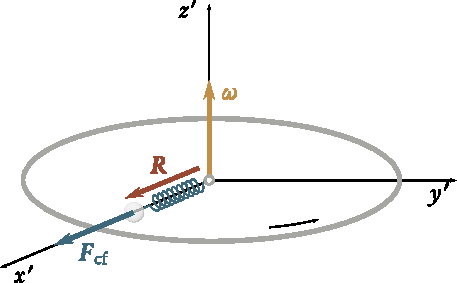
\includegraphics[scale=0.95]{figures/ch_04/fig_4_3.pdf}
		\caption[]{}
		\label{fig:4_3}
	\end{center}
\end{figure}

Quả cầu là đứng yên đối với hệ quy chiếu gắn với đĩa. Có thể giải thích một cách hình thức điều này là ngoài lực~\eqref{eq:4_4} còn có lực quán tính
\begin{equation}\label{eq:4_5}
\vec{F}_{\text{cf}} = m\omega^2\vec{R}.
\end{equation}

\noindent
hướng dọc theo bán kính tính từ tâm đĩa tác dụng lên quả cầu.

Người ta gọi lực quán tính~\eqref{eq:4_5} xuất hiện trong hệ quy chiếu quay (đối với các hệ quán tính) là \textit{lực quán tính ly tâm}. Trong hệ quy chiếu quay, lực này tác dụng lên vật và không phụ thuộc vào việc vật đang đứng yên đối với hệ (như ta đã giả thiết cho đến bây giờ) hoặc chuyển động đối với nó với vận tốc $\vec{v}'$.

\begin{figure}[!htb]
	\begin{minipage}[t]{0.5\linewidth}
		\begin{center}
			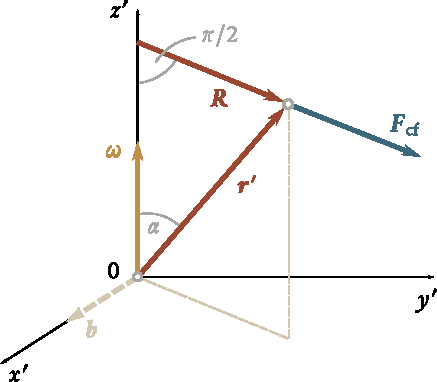
\includegraphics[scale=0.6]{figures/ch_04/fig_4_4.pdf}
			\caption[]{}
			\label{fig:4_4}
		\end{center}
	\end{minipage}
	\hspace{-0.05cm}
	\begin{minipage}[t]{0.5\linewidth}
		\begin{center}
			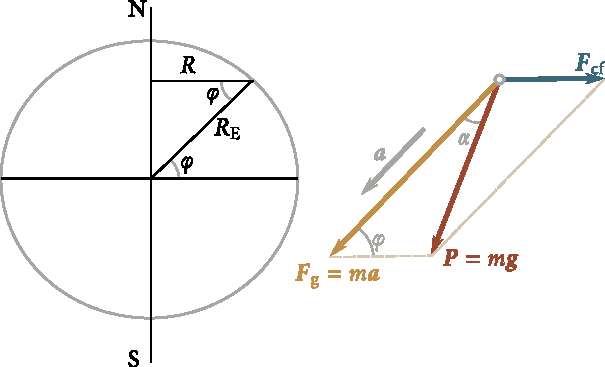
\includegraphics[scale=0.6]{figures/ch_04/fig_4_5.pdf}
			\caption[]{}
			\label{fig:4_5}
		\end{center}
	\end{minipage}
\end{figure}

Nếu vị trí của vật trong hệ quy chiếu quay được đặc trưng bởi vector vị trí $\vec{r}'$, lực ly tâm khi đó có thể được biểu diễn dưới dạng tích vector kép
\begin{equation}\label{eq:4_6}
\vec{F}_{\text{cf}} = m [\vec{\omega} \times (\vec{r}'\times\vec{\omega})].
\end{equation}

\noindent
Thực vậy, vector $\vec{b}=\vec{r}'\times\vec{\omega}$ hướng vuông góc với các vector $\vec{\omega}$ và $\vec{F}_{\text{cf}}$ ``tới chúng ta'' (\fig{4_4}), và có độ lớn bằng $\omega r'\sin\alpha=\omega R$. Tích vector của các vector vuông góc với nhau $m\vec{\omega}$ và $\vec{b}$ trùng với $\vec{F}_{\text{cf}}$ về hướng, có độ lớn bằng $m\omega b=m\omega^2R=\vec{F}_{\text{cf}}$.

Khi giải chính xác bài toán về chuyển động của các vật đối với mặt đất, ta cần phải coi lực quán tính ly tâm bằng $m\omega^2R$, trong đó $m$ là khối lượng của vật, $\omega$ là vận tốc góc quay của Trái đất xung quanh trục của nó, và $R$ là khoảng cách của vật tới trục của Trái đất (\fig{4_5}). Trong trường hợp độ cao của các vật trên mặt đất không lớn, có thể đặt $R=R_{\text{E}}\cos\varphi$ ($R_{\text{E}}$ là bán kính Trái đất, và $\varphi$ là vĩ độ của khu vực). Biểu thức mô tả lực quán tính ly tâm khi đó có dạng
\begin{equation}\label{eq:4_7}
F_{\text{cf}} = m\omega^2 R_{\text{E}}\cos\varphi.
\end{equation}

Gia tốc rơi tự do $\vec{g}$ của các vật được quan sát đối với Trái đất được gây bởi tác dụng của lực $\vec{F}_{\text{g}}$ mà vật bị Trái đất hút, và lực $\vec{F}_{\text{cf}}$. Lực tổng hợp của các lực này
\begin{equation}\label{eq:4_8}
\vec{P} = \vec{F}_{\text{g}} + \vec{F}_{\text{cf}}
\end{equation}

\noindent
là trọng lực bằng $m\vec{g}$ [xem \eqn{2_38}].

Sai khác giữa trọng lực $\vec{P}$ với lực hút $\vec{F}_{\text{g}}$ tới Trái đất là không lớn, vì lực quán tính ly tâm nhỏ hơn $\vec{F}_{\text{g}}$ rất nhiều. Chẳng hạn với một vật khối lượng \SI{1}{\kilo\gram}, giá trị lớn nhất của $F_{\text{cf}}$ quan sát trên xích đạo bằng
\begin{equation*}
m\omega^2 R_{\text{E}} = 1 \times \left(\frac{2\pi}{86400}\right)^2 \times \num{6.4e6} = \SI{0.035}{\newton}
\end{equation*}

\noindent
trong khi $\vec{F}_{\text{g}}$ gần bằng \SI{9.8}{\newton}, nghĩa là lớn hơn gần $300$ lần.

Có thể xác định góc $\alpha$ giữa hướng của $\vec{F}_{\text{g}}$ và $\vec{P}$ (xem \fig{4_5}) khi dùng định lý sin:
\begin{equation*}
\frac{\sin\alpha}{\sin\varphi} = \frac{F_{\text{g}}}{P} = \frac{m\omega^2 R_{\text{E}}\cos\varphi}{mg} \approx \frac{\SI{0.035}{\newton}}{\SI{9.8}{\newton}} \cos\varphi \approx 0.0035 \cos\varphi
\end{equation*}

\noindent
từ đó
\begin{equation*}
\sin\alpha \approx 0.0035\sin\varphi\cos\varphi \approx 0.0018 \sin 2\varphi.
\end{equation*}

\noindent
Sin của một góc nhỏ có thể được thay một cách gần đúng bằng giá trị của chính góc đó. Kết quả ta có
\begin{equation}\label{eq:4_9}
\alpha \approx 0.0018 \sin 2\varphi.
\end{equation}

\noindent
Như vậy góc $\alpha$ biến đổi trong phạm vi từ không (ở xích đạo, tại đó $\varphi=0$, và ở các các cựcand at the poles, tại đó $\varphi=\SI{90}{\degree}$) đến \SI{0.0018}{\radian} hoặc $6'$ (tại vĩ độ \SI{45}{\degree}).

Hướng của lực $\vec{P}$ trùng với hướng của sợi dây bị căng bởi quả nặng, được gọi là hướng dây dọi hoặc hướng thẳng đứng. Lực $\vec{F}_{\text{g}}$ hướng vào tâm Trái đất. Do đó, đường thẳng đứng hướng vào tâm Trái đất chỉ khi ở các cực hoặc ở xích đạo, còn ở các vĩ độ trung gian thì bị lệch một góc $\alpha$ xác định bởi biểu thức~\eqref{eq:4_9}.

Hiệu $F_{\text{g}}-P$ bằng không ở các cực và đạt cực đại bằng $0.3$\% lực $F_{\text{g}}$ tại xích đạo. Vì Trái đất bị dẹt ở các cực nên lực $F_{\text{g}}$ tự nó sẽ biến đổi một ít theo vĩ độ, ở xích đạo nhỏ hơn ở các cực khoảng $0.2$\%. Kết quả là gia tốc rơi tự do biến thiên với vĩ độ trong phạm vi từ \SI{9.780}{\metre\per\square\second} ở xích đạo đến \SI{9.832}{\metre\per\square\second} ở các cực. Giá trị $g=\SI{9.80665}{\metre\per\square\second}$ được lấy làm giá trị tiêu chuẩn.

Ta cần chú ý rằng đối với hệ quy chiếu quán tính, chẳng hạn hệ quy chiếu nhật tâm, vật rơi tự do thì chuyển động với gia tốc $\vec{a}=\vec{F}_{\text{g}}/m$ (mà không phải $\vec{g}$). Từ \fig{4_5}, rõ ràng là từ sự bằng nhau của gia tốc $g$ đối với các vật khác nhau ta suy ra được sự bằng nhau của các gia tốc $a$. Thật vậy, các tam giác được tạo thành từ các vector $\vec{F}_{\text{g}}$ và $\vec{P}$ đối với các vật khác nhau đều đồng dạng với nhau (các góc $\alpha$ và $\varphi$ đối với mọi vật tại một điểm đã cho của mặt đất đều như nhau). Do đó, tỷ số $F_{\text{g}}/P$, trùng với tỷ số $a/g$, đối với mọi vật đều như nhau. Từ đó suy ra rằng các $a$ như nhau với các $g$ như nhau.

\section{Lực Coriolis}\label{sec:4_3}

Khi một vật chuyển động trong một hệ quy chiếu quán tính quay, ngoài lực quán tính ly tâm còn xuất hiện một lực khác gọi là \textbf{lực Coriolis} hay \textbf{lực quán tính Coriolis}.

Có thể phát hiện sự xuất hiện của lực quán tính Coriolis trong thí nghiệm sau. Ta lấy một đĩa được đặt nằm ngang có thể quay xung quanh một trục thẳng đứng. Ta vẽ trên đĩa đường thẳng $OA$ đi qua tâm đĩa (\fig{4_6}a). Ta ném một quả cầu với vận tốc $\vec{v}'$ theo hướng từ $0$ đến $A$. Nếu đĩa không quay, quả cầu sẽ trượt dọc theo đường thẳng ta đã vẽ trước đó. Tuy nhiên, nếu đĩa quay theo chiều mũi tên thì quả cầu sẽ trượt dọc theo đường cong $OB$ được vẽ nét đứt, trong khi đó vận tốc $\vec{v}'$ của nó đối với đĩa sẽ đổi hướng. Do đó đối với hệ quy chiếu quay, quả cầu chuyển động như thể có lực $\vec{F}_{\text{Cor}}$ vuông góc với $\vec{v}'$ tác dụng lên quả cầu.

\begin{figure}[!htb]
	\begin{center}
		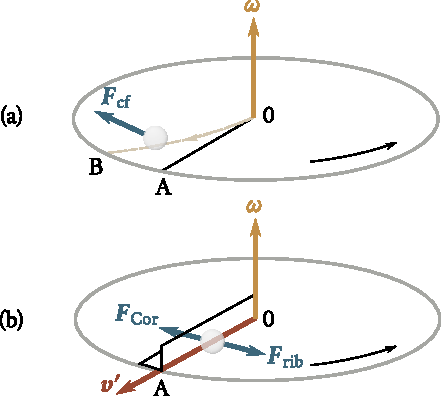
\includegraphics[scale=1]{figures/ch_04/fig_4_6.pdf}
		\caption[]{}
		\label{fig:4_6}
	\end{center}
\end{figure}

Để bắt quả cầu trượt trên đĩa quay dọc theo một đường thẳng đi qua tâm, ta phải thiết lập một đường chuẩn, dưới dạng chẳng hạn như cạnh $0A$ (\fig{4_6}b). Khi quả cầu đang lăn, cạnh chuẩn tác dụng lên nó một lực $\vec{F}_{\text{rib}}$ nào đó. Đối với hệ quy chiếu quay (gắn với đĩa), quả cầu chuyển động với vận tốc có hướng không đổi. Có thể giải thích một cách hình thức điều này là, lực  $\vec{F}_{\text{rib}}$ cân bằng với lực quán tính $\vec{F}_{\text{Cor}}$ vuông góc với $\vec{v}'$ tác dụng lên quả cầu. Chính lực $\vec{F}_{\text{Cor}}$ là lực quán tính Coriolis.

Trước hết ta đi tìm biểu thức của lực Coriolis đối với trường hợp riêng khi đối với hệ quy chiếu quay, hạt $m$ chuyển động đều theo một đường tròn nằm trong mặt phẳng vuông góc với trục quay có tâm nằm trên trục này (\fig{4_7}). Đặt $\vec{v}'$ là vận tốc của hạt đối với hệ quay. Vận tốc của hạt đối với hệ quy chiếu (quán tính) đứng yên là $\vec{v}$, về độ lớn bằng $v'+\omega R$ trong trường hợp (a) và $|v-\omega R|$ trong trường hợp (b), trong đó $\omega$ là vận tốc góc của hệ quay, và $R$ là bán kính của đường tròn [xem \eqn{1_99}].

\begin{figure}[!htb]
	\begin{center}
		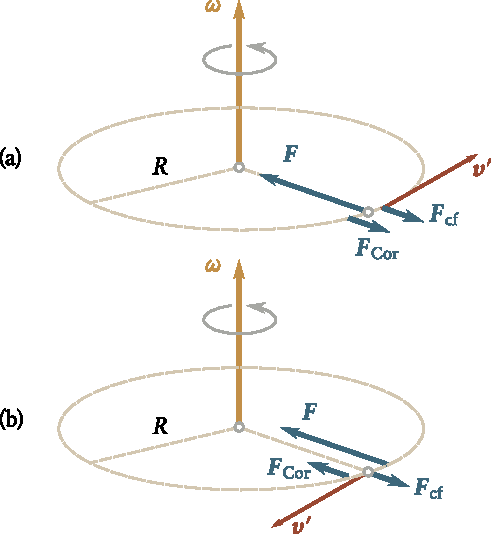
\includegraphics[scale=1]{figures/ch_04/fig_4_7.pdf}
		\caption[]{}
		\label{fig:4_7}
	\end{center}
\end{figure}

Để hạt chuyển động theo một đường tròn với vận tốc $v=v'+\omega R$ đối với hệ đứng yên, nó cần phải chịu tác dụng của một lực $\vec{F}$ hướng vào tâm đường tròn, chẳng hạn như lực căng của sợi dây buộc hạt với tâm đường tròn (xem \fig{4_7}a). Độ lớn của lực này bằng
\begin{equation}\label{eq:4_10}
F = m a_{\hatvec{n}} = \frac{mv^2}{R} = \frac{m(v'+\omega R)^2}{R} = \frac{mv'^2}{R} + 2mv'\omega + m\omega^2 R.
\end{equation}

\noindent
Đối với hệ quay, hạt trong trường hợp này chuyển động với gia tốc $a_{\hatvec{n}}'=v'^2/R$, như thế có lực
\begin{equation}\label{eq:4_11}
m a_{\hatvec{n}}' = \frac{mv^2}{R} = F - 2mv'\omega - m\omega^2 R
\end{equation}

\noindent
tác dụng lên nó [xem \eqn{4_10}]. Như vật trong hệ quy chiếu quay, hạt thể hiện đúng như thể ngoài lực $\vec{F}$ hướng về tâm đường tròn còn có hai lực hướng ra xa tâm tác dụng lên nó. Hai lực này là $\vec{F}_{\text{cf}}=m\omega^2 R$ và $\vec{F}_{\text{Cor}}$ có độ lớn bằng $2mv'\omega$ (\fig{4_7}a). Dễ dàng thấy được rằng có thể biểu diễn lực $\vec{F}_{\text{Cor}}$ dưới dạng
\begin{equation}\label{eq:4_12}
\vec{F}_{\text{Cor}} = 2m(\vec{v}'\times\vec{\omega}).
\end{equation}

\noindent
Lực~\eqref{eq:4_12} chính là lực quán tính Coriolis. Khi $\vec{v}'=0$ lực này bị triệt tiêu. Lực $\vec{F}_{\text{cf}}$ không phụ thuộc vào $\vec{v}'$---như ta đã chỉ ra, nó tác dụng cả lên vật đứng yên lẫn vật chuyển động.

Trong trường hợp vẽ trên hình \fig{4_7}b, ta có
\begin{equation*}
	F = \frac{mv^2}{R} = \frac{m(v'-\omega R)^2}{R} = \frac{mv'^2}{R} - 2mv'\omega + m\omega^2 R.
\end{equation*}

\noindent
Một cách tương ứng,
\begin{equation*}
\frac{mv'^2}{R} = F + 2mv'\omega - m\omega^2 R.
\end{equation*}

\noindent
Do đó trong hệ quay, hạt thể hiện như thể có hai lực $\vec{F}$ và $\vec{F}_{\text{Cor}}$ tác dụng hướng về tâm đường tròn, và cả lực $\vec{F}_{\text{cf}}=m\omega^2R$ hướng ra xa tâm (xem \fig{4_7}b). Chính lực $\vec{F}_{\text{Cor}}$ trong trường hợp này có thể được biểu diễn dưới dạng \eqn{4_12}.

\begin{figure}[!htb]
	\begin{center}
		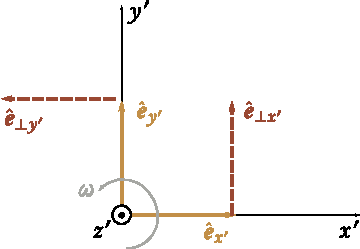
\includegraphics[scale=1]{figures/ch_04/fig_4_8.pdf}
		\caption[]{}
		\label{fig:4_8}
	\end{center}
\end{figure}

Bây giờ ta chuyển sang tìm biểu thức của lực Coriolis đối với trường hợp khi hạt chuyển động đối với hệ quy chiếu quay tùy ý. Ta gắn các trục tọa độ $x', y', z'$ với hệ quay và cho trục $z'$ trùng với trục quay (\fig{4_8}). vector vị trí của hạt có thể được biểu diễn dưới dạng
\begin{equation}\label{eq:4_13}
\vec{r}' = x'\vecuni{x}' + y'\vecuni{y}' + z'\vecuni{z}'
\end{equation}

\noindent
trong đó $\vecuni{x}'$, $\vecuni{y}'$ và $\vecuni{z}'$ là các vector đơn vị của các trục tọa độ. Các vector đơn vị $\vecuni{x}'$ và $\vecuni{y}'$ quay cùng với hệ quy chiếu với vận tốc góc $\omega$, trong khi vector đơn vị $\vecuni{z}'$ không chuyển động.

Ta cần phải xác định vị trí của hạt đối với hệ đứng yên nhờ vector vị trí $\vec{r}$. Tuy nhiên, các ký hiệu $\vec{r}'$ and $\vec{r}$ đại diện cho cùng một vector vẽ từ gốc tọa độ đến hạt. Một người quan sát ``sống'' trong hệ quy chiếu quay đã ký hiệu vector này bằng $\vec{r}'$. Theo sự quan sát của anh ta, các vector đơn vị $\vecuni{x}'$, $\vecuni{y}'$ và $\vecuni{z}'$ đều đứng yên, do đó khi lấy vi phân biểu thức \eqn{4_13} anh ta coi các vector đơn vị này như các hằng số. Người quan sát đứng yên sử dụng ký hiệu $\vec{r}$. Đối với anh ta, các vector đơn vị $\vecuni{x}'$ và $\vecuni{y}'$ quay với vận tốc góc $\omega$ (vector đơn vị $\vecuni{z}'$ không chuyển động). Do đó, khi lấy vi phân~\eqref{eq:4_13} bằng $\vec{r}$, anh ta phải coi $\vecuni{x}'$ và $\vecuni{y}'$ như các hàm của $t$ có các đạo hàm:
\begin{equation}\label{eq:4_14}
\dot{\hatvec{e}}_x' = \omega\vecuni{y}',\quad \dot{\hatvec{e}}_y' = -\omega\vecuni{x}'
\end{equation}

\noindent
[xem \fig{4_8} và \eqn{1_56}; vector đơn vị $\vecuni{\perp x'}$ vuông góc với $\vecuni{x}'$ bằng $\vecuni{y}'$ và vector đơn vị $\vecuni{\perp y'}$ vuông góc với $\vecuni{y'}$ bằng $-\vecuni{x'}$]. Đối với đạo hàm bậc hai của các vector đơn vị theo thời gian, ta thu được các biểu thức:
\begin{equation}\label{eq:4_15}
\ddot{\hatvec{e}}_x' = \omega\dot{\hatvec{e}}_y' = -\omega^2\vecuni{x}',\quad \ddot{\hatvec{e}}_y' = \omega\dot{\hatvec{e}}_x' = -\omega^2\vecuni{y}'.
\end{equation}

Ta tìm vận tốc của hạt đối với hệ quy chiếu quay. Muốn vậy, ta lấy vi phân vector vị tri~\eqref{eq:4_13} theo thời gian, nếu coi các vector đơn vị là hằng số:
\begin{equation}\label{eq:4_16}
\vec{v}' = \dot{\vec{r}}' = \dot{x}'\vecuni{x}' + \dot{y}'\vecuni{y}' + \dot{z}'\vecuni{z}'
\end{equation}

\noindent
Lấy vi phân lần nữa biểu thức này, ta được gia tốc của hạt đối với hệ quy chiếu quay:
\begin{equation}\label{eq:4_17}
\vec{a}' = \dot{\vec{v}}' = \ddot{\vec{r}}' = \ddot{x}'\vecuni{x}' + \ddot{y}'\vecuni{y}' + \ddot{z}'\vecuni{z}'.
\end{equation}

Bây giờ ta tìm vận tốc của hạt đối với hệ quy chiếu đứng yên. Muốn vậy, ta lấy vi phân vector vị trí~\eqref{eq:4_13} ``theo quan điểm'' của người quan sát đứng yên. Dùng ký hiệu $\vec{r}$ thay cho $\vec{r}'$ (nhớ rằng $\vec{r}=\vec{r}'$), ta có:
\begin{equation}\label{eq:4_18}
\vec{v} = \dot{\vec{r}} = \dot{x}'\vecuni{x}' + x'\dot{\hatvec{e}}_x' + \dot{y}'\vecuni{y}' + y'\dot{\hatvec{e}}_y' + \dot{z}'\vecuni{z}' + z'\dot{\hatvec{e}}_z'.
\end{equation}

\noindent
Lấy vi phân biểu thức này theo $t$ một lần nữa, ta tìm được gia tốc của hạt đối với hệ đứng yên:
\begin{equation*}
\vec{a} = \dot{\vec{v}} =
\ddot{x}'\vecuni{x}' + 2\dot{x}'\dot{\hatvec{e}}_x' + x'\ddot{\hatvec{e}}_y' + \ddot{y}'\vecuni{y}' + 2\dot{y}'\dot{\hatvec{e}}_y' + y'\ddot{\hatvec{e}}_y' + \ddot{z}'\vecuni{z}' + 2\dot{z}'\dot{\hatvec{e}}_z' + z'\ddot{\hatvec{e}}_z'.
\end{equation*}

\noindent
Nếu để ý tới các công thức~\eqref{eq:4_14}, \eqref{eq:4_15}, và \eqref{eq:4_17}, ta có thể biến đổi hệ thức thu được về dạng:
\begin{equation}\label{eq:4_19}
\vec{a} = \vec{a}' + 2\omega(\dot{x}'\vecuni{y}' - \dot{y}\vecuni{x}') - \omega^2(x'\vecuni{x}' + \dot{y}\vecuni{y}').
\end{equation}

Ta hãy xét tích vector $\vecprod{\omega}{v}'$. Ta biểu diễn nó dưới dạng một định thức [xem \eqn{1_33}]:
\begin{equation}\label{eq:4_20}
\vecprod{\omega}{v}' = \begin{vmatrix}
\vecuni{x}' & \vecuni{y}' & \vecuni{z}'\\
\omega_x & \omega_y & \omega_z\\
v_x' & v_y' & v_z'
\end{vmatrix}.
\end{equation}

\noindent
Theo \eqn{4_16}, $v_x=\dot{x}', v_y=\dot{y}', v_z=\dot{z}'$. Ngoài ra, với hướng của các trục tọa độ mà ta đã chọn, ta có $\omega_x=\omega_y=0, \omega_z=\omega$. Thay các giá trị này vào \eqn{4_20} ta được
\begin{equation}\label{eq:4_21}
\vecprod{\omega}{v}' = \begin{vmatrix}
\vecuni{x}' & \vecuni{y}' & \vecuni{z}'\\
0 & 0 & \omega\\
\dot{x}' & \dot{y}' & \dot{z}'
\end{vmatrix} = -\vecuni{x}'\omega\dot{y}' + \vecuni{y}'\omega\dot{x}'.
\end{equation}

\noindent
Kết quả thu được chứng tỏ rằng có thể viết số hạng thứ hai của công thức \eqn{4_19} dưới dạng $2\vecprod{\omega}{v}'$. Biểu thức đứng trong các dấu ngoặc ở số hạng cuối của \eqn{4_19} bằng với thành phần vuông góc với trục quay (trục $z'$) của vector vị trí $\vec{r}'$ [xem \eqn{4_13}]. Ta ký hiệu thành phần này bằng $\vec{R}$ (so sánh với \fig{1_33}). Nếu chú ý tới tất cả những điều đã nói trước đó, \eqn{4_19} có thể được viết lại như sau:
%\vspace{-12pt}
\begin{equation}\label{eq:4_22}
\vec{a} = \vec{a}' + 2\vecprod{\omega}{v}' - \omega^2\vec{R}.
\end{equation}

Từ \eqn{4_22} ta suy ra rằng gia tốc của hạt đối với hệ quy chiếu đứng yên có thể được biểu diễn dưới dạng tổng của ba gia tốc: gia tốc $\vec{a}'$ đối với hệ quay, gia tốc bằng $-\omega^2\vec{R}$\footnote{Gia tốc $\vec{a}_{\text{tr}}=-\omega^2\vec{R}$ được gọi là gia tốc chuyển. Nó là gia tốc mà hạt đứng yên trong hệ quy chiếu chuyển động (trong trường hợp của ta là hệ quy chiếu quay) đã có.}, và gia tốc
\begin{equation}\label{eq:4_23}
\vec{a}_{\text{Cor}} = 2\vecprod{\omega}{v}'
\end{equation}

\noindent
được gọi là \textbf{gia tốc Coriolis}.

Để hạt chuyển động với gia tốc~\eqref{eq:4_22}, các vật phải tác dụng lên nó một lực tổng hợp $\vec{F}=m\vec{a}$. Theo \eqn{4_22}
\begin{equation}\label{eq:4_24}
m\vec{a}' = m\vec{a} - 2m\vecprod{\omega}{v}' + m\omega^2\vec{R} = \vec{F} + 2m\vec{v}'\times\vec{\omega} + m\omega^2\vec{R}
\end{equation}

\noindent
(sự hoán vị giữa các thừa số sẽ làm thay đổi dấu của tích vector). Kết quả thu được có nghĩa là khi lập phương trình của định luật Newton thứ hai trong hệ quy chiếu quay, ngoài các lực tương tác, cần phải tính đến lực quán tính ly tâm xác định bởi \eqn{4_25}, và cả lực Coriolis mà ngay trong trường hợp tổng quát nhất được xác định bởi \eqn{4_12}. Ta chú ý rằng lực Coriolis luôn luôn nằm trong mặt phẳng vuông góc với trục quay.

Từ sự so sánh các biểu thức~\eqref{eq:4_14}, \eqref{eq:4_16}, và \eqref{eq:4_18} ta có
\begin{equation*}
\vec{v} = \vec{v}' + x'\dot{\hatvec{e}}_x' + y'\dot{\hatvec{e}}_y' = \vec{v}' + \omega(x'\vecuni{y}' - y'\vecuni{x}').
\end{equation*}

\noindent
Các tính toán tương tự dẫn ta tới \eqn{4_22} có thể khẳng định rằng số hạng cuối của biểu thức thu được là bằng $\vecprod{\omega}{v}'$. Do đó,
\begin{equation}\label{eq:4_25}
\vec{v} = \vec{v}' + \vecprod{\omega}{v}'.
\end{equation}

\noindent
Với $\vec{v}'=0$, biểu thức này chuyển thành \eqn{1_100}.

\begin{figure}[!htb]
	\begin{minipage}[t]{0.34\linewidth}
		\begin{center}
			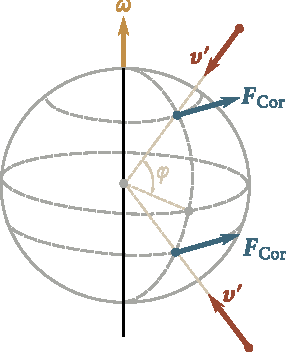
\includegraphics[scale=0.84]{figures/ch_04/fig_4_9.pdf}
			\caption[]{}
			\label{fig:4_9}
		\end{center}
	\end{minipage}	
	\hspace{-0.05cm}
	\begin{minipage}[t]{0.34\linewidth}
		\begin{center}
			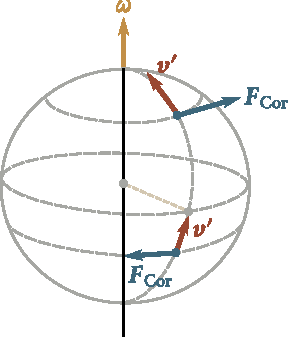
\includegraphics[scale=0.84]{figures/ch_04/fig_4_10.pdf}
			\caption[]{}
			\label{fig:4_10}
		\end{center}
	\end{minipage}
	\hspace{-0.2cm}
	\begin{minipage}[t]{0.3\linewidth}
		\begin{center}
			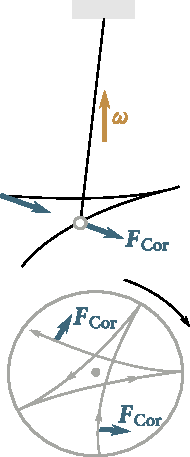
\includegraphics[scale=0.84]{figures/ch_04/fig_4_11.pdf}
			\caption[]{}
			\label{fig:4_11}
		\end{center}
	\end{minipage}
\end{figure}

\textbf{Các ví dụ về các chuyển động trong đó có xuất hiện lực quán tính Coriolis.} Khi giải thích các hiện tượng liên quan tới sự chuyển động của các vật đối với mặt đất, ta cần phải tính đến ảnh hưởng của các lực Coriolis trong một số trường hợp. Chẳng hạn, trong quá trình rơi tự do của các vật thì lực Coriolis tác dụng lên chúng sẽ gây ra sự lệch sang phía Đông của dây rọi (\fig{4_9}). Lực này ảnh hưởng cực đại ở xích đạo và triệt tiêu ở các cực.

Một viên đạn bay cũng chịu các độ lệch gây ra bởi các lực quán tính Coriolis (\fig{4_10}). Khi bắn một phát đại bác hướng về phía Bắc, viên đạn sẽ lệch sang phía đông ở Bắc Bán cầu và lệch sang phía Tây ở Nam Bán cầu. Khi bắn dọc theo đường kinh tuyến xuống phía Nam, các phương lệch sẽ ngược lại. Khi bắn dọc theo xích đạo, lực Coriolis sẽ ép viên đạn xuống đất nếu bắn về hướng Tây, và nâng viên đạn lên nếu bắn về hướng Đông. Chúng tôi nhường cho độc giả tự khẳng định rằng lực Coriolis tác dụng lên vật chuyển động dọc theo đường kinh tuyến theo một hướng bất kỳ (hướng Bắc hoặc hướng Nam) sẽ hướng sang phải ở Bắc Bán cầu và sang trái ở Nam Bán cầu đối với hướng chuyển động. Đây là lý do vì sao những con sông luôn bị xói mòn bờ bên phải nếu ở Bắc Bán cầu và bờ bên trái nếu ở Nam bán cầu. Đồng thời đó cũng là lý do vì sao những đường ray dùng cho tàu lửa chuyển động bị mài mòn không đồng đều.

Các lực Coriolis cũng xuất hiện trong dao động của con lắc. Hình~\ref{fig:4_11} biểu diễn quỹ đạo của vật nặng của con lắc (để đơn giản, giả sử con lắc nằm tại một cực của Trái Đất). Ở Bắc cực, lực Coriolis luôn hướng sang phải theo chiều chuyển động của con lắc, còn ở Nam cực thì hướng sang phải. Kết quả là quỹ đạo của con lắc có dạng tán đèn hình phễu.

Có thể nhìn thấy từ hình vẽ, mặt phẳng dao động của con lắc quay theo chiều kim đồng hồ đối với Trái Đất, đồng thời nó thực hiện được một vòng trong một ngày đêm. Đối với hệ quy chiếu nhật tâm, mặt phẳng dao động ở trạng thái nghỉ còn Trái Đất quay được một vòng trong một ngày đêm. Có thể chứng tỏ rằng ở ví độ $\varphi$, mặt phẳng dao động của con lắc quay trong một ngày đêm một góc $2\pi\sin\varphi$.

Như vậy, các quan sát về sự quay mặt phẳng dao động của con lắc (các con lắc được dùng vào việc này được gọi là các con lắc Foucault) chứng minh trực tiếp sự quay của Trái đất xung quanh trục của nó.

\section{Các định luật bảo toàn trong hệ quy chiếu phi quán tính}\label{sec:4_4}

Nếu để ý tới các lực quán tính thì các phương trình chuyển động trong hệ phi quán tính không có gì khác so với các phương trình chuyển động trong hệ quy chiếu quán tính. Do đó, mọi kết luận rút ra từ các phương trình chuyển động, cụ thể là các hệ thức~\eqref{eq:3_77}, \eqref{eq:3_88}, và \eqref{eq:3_118}, vẫn đúng cả trong hệ quy chiếu không quán tính.

\begin{figure}[!htb]
	\begin{center}
		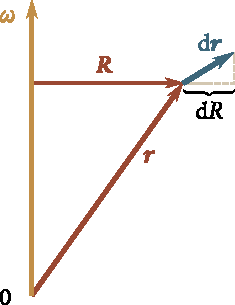
\includegraphics[scale=1]{figures/ch_04/fig_4_12.pdf}
		\caption[]{}
		\label{fig:4_12}
	\end{center}
\end{figure}

Trong hệ phi quán tính, công thức~\eqref{eq:3_77} có dạng:
\begin{equation}\label{eq:4_26}
E_2-E_1 = A_{12,\text{non-cons}} + A_{12,\text{in}}
\end{equation}

\noindent
trong đó $A_{12,\text{in}}$ là công của các lực quán tính.

Các công thức~\eqref{eq:3_88} và ~\eqref{eq:3_118} hiện ra trong hệ không quán tính như sau:
\begin{align}
\diff{\vec{p}}{t} &= \sum\vec{F}_{\text{ext}} + \sum\vec{F}_{\text{in}}\label{eq:4_27}\\
\diff{\vec{L}}{t} &= \sum\vec{M}_{\text{ext}} + \sum\vec{M}_{\text{in}}\label{eq:4_28}.
\end{align}

Ở đây $\vec{F}_{\text{ext}}$ là lực gây ra bởi tương tác, $\vec{F}_{\text{in}}$ là lực quán tính, $\vec{M}_{\text{ext}}$ và $\vec{M}_{\text{in}}$ là các moment của các lực đã nêu.

Lực quán tính ly tâm $\vec{F}_{\text{cf}}=m\omega^2 R$ là lực bảo toàn. Thực vậy, công của lực này bằng
\begin{equation*}
A_{12,\text{cf}} = \int_1^2\vec{F}_{\text{cf}}\,\deriv{\vec{r}} = m\omega^2\int_{1}^{2}\vec{R}\,\deriv{\vec{r}}.
\end{equation*}

\noindent
Từ~\fig{4_12}, hình chiếu của vector $\deriv{\vec{r}}$ lên hướng của vector $\vec{R}$ bằng $\deriv{R}$---số gia của module của $\vec{R}$. Do đó, $\vec{R}\deriv{\vec{r}}=R\,\deriv{R} = \deriv{R^2/2}$. Như vậy,
\begin{equation}\label{eq:4_29}
A_{12,\text{cf}} = m\omega^2 \int_{1}^{2} \deriv{R^2/2} = m\omega^2 \frac{R^2_2}{2} - m\omega^2 \frac{R^2_1}{2}.
\end{equation}

\noindent
Biểu thức thu được rõ ràng không phụ thuộc vào quãng đường theo đó sự dịch chuyển từ điểm $1$ đến điểm $2$ đã xảy ra.

Tính chất bảo toàn của lực $\vec{F}_{\text{cf}}$ cho phép đưa vào thế năng $E_{\text{p,cf}}$ của hạt (năng lượng ly tâm), mà độ giảm của nó xác định công của lực quán tính ly tâm:
\begin{equation}\label{eq:4_30}
A_{12,\text{cf}} = E_{\text{p,cf},1} - E_{\text{p,cf},2}
\end{equation}

\noindent
[xem \eqn{3_30}]. Từ sự so sánh các công thức~\eqref{eq:4_29} và \eqref{eq:4_30} ta kết luận rằng $E_{\text{p,cf}}=-m\omega^2R^2/2 + \text{constant}$. Ta có thể đặt hằng số bằng không. Khi đó đối với năng lượng ly tâm ta thu được biểu thức sau:
\begin{equation}\label{eq:4_31}
E_{\text{p,cf}} = -\frac{1}{2} m \omega^2 R^2.
\end{equation}

Nếu ta bổ sung \eqn{4_31} vào thế năng của hạt thì không cần phải đưa công của lực quán tính ly tâm vào đại lượng $A_{12,\text{in}}$ trong công thức \eqn{4_26}.